\documentclass[10pt]{article}

\usepackage[T1]{fontenc}
\usepackage[utf8]{inputenc}
\usepackage{lmodern}
\usepackage[margin=0.85in]{geometry}
\usepackage{amsmath,amssymb}
\usepackage{booktabs}
\usepackage{float}
\usepackage{graphicx}
\usepackage{xcolor}
\usepackage{tikz}
\usetikzlibrary{arrows.meta,positioning,fit,calc,shapes.geometric}
\usepackage[hidelinks]{hyperref}

\renewcommand{\topfraction}{0.9}
\renewcommand{\bottomfraction}{0.6}
\renewcommand{\textfraction}{0.08}
\renewcommand{\floatpagefraction}{0.8}
\setcounter{topnumber}{3}
\setcounter{bottomnumber}{2}
\setcounter{totalnumber}{5}

\newcommand{\pfail}{p_{\mathrm{fail}}}
\newcommand{\dc}{d_{\mathrm c}}
\newcommand{\vecop}{\operatorname{vec}}
\newcommand{\dd}{\mathrm{d}}
\newcommand{\Pcomp}{\Pi_{\mathrm c}}

\title{Physical-Level Noise for Circuit Learning:\\
Spectral Master-Equation Solves, Leakage-Aware Gate Control,\\
Device Cards, and Evolutionary Circuit Search}

\author{Ryan Vogt\thanks{Rochester Institute of Technology. Technical
overview prepared for collaborators, including T.~Desell (EXAQC); status as
of 20 October 2026. All numbers are taken from the campaign records named in
the text; results marked preliminary are preliminary.}}

\date{20 October 2026}

\begin{document}

\maketitle

\begin{abstract}
This report describes a research program that couples four computational
layers which are usually developed in isolation: a spectral-element solver in
time for open-system quantum master equations, including equations with a
memory kernel; gate-level optimal control of transmon gates in which the
leakage levels are retained and penalized; a compact per-gate summary of each
optimized gate, which we call a device card; and a multi-objective genetic
algorithm, built on the EXAQC framework, that evolves circuits against a noise
model read from the card. The aim is to make learned circuits answerable to
the device on which they will run, and to make the device model a variable
that one can change. We describe each layer in enough detail for a reader
outside quantum control to follow the argument, report the results obtained so
far, and state plainly which of them are preliminary. In brief: single-qubit
cards at five transmon levels are complete; the two-qubit CNOT cards are not yet
trustworthy, because a four-level truncation is insufficient and the device
we had been using places a frequency collision inside the drive band; and the
circuit-level results to date show that conditioning the search on the card
helps where the card carries information that a uniform error model lacks,
chiefly bath memory, and that most of the remaining gain over textbook circuits
is depth reduction of the kind a compiler already performs.
\end{abstract}

\section{Introduction}
\label{sec:intro}

A circuit that is cheap by the usual metrics need not be cheap on hardware.
Gate count, two-qubit gate count and depth are proxies for the error a circuit
accumulates, and each proxy is calibrated against a picture of the device in
which every gate of a given arity costs the same and idling costs nothing.
Superconducting devices violate this picture in ways that matter at the
circuit level. A two-qubit gate takes several times as long as a single-qubit
gate, so that a shallow circuit dense in entanglers can leave its spectators
idle for longer than a deeper circuit that spreads the work out. Gates of equal
average fidelity can have different error channels, and the composition of two
biased channels is not the composition of two depolarizing channels. Under a
bath with memory an idle qubit and a driven qubit are not interchangeable at
all.

Optimal control supplies precisely the information these proxies discard.
Given a device Hamiltonian, control operators, bounds on the drive and a
dissipative model, one can compute the pulse that realizes a target gate and
the channel that pulse actually implements, including the part of the error
that leaves the computational subspace. That computation is expensive, and it
is almost always reported as one number, the gate infidelity, which is exactly
the reduction that throws away what the circuit level needs.

In this report we describe a pipeline that keeps that information and passes
it upward. The pipeline is shown in Figure~\ref{fig:pipeline}. At the bottom is
a master equation for a pair of transmons, in one of four models of the
environment. We solve it with spectral collocation in time, segment by segment,
and we differentiate the solution exactly by one transposed solve. On top of
the solver sits a gate-level control problem, solved by L-BFGS with that
adjoint gradient, whose cost carries a leakage penalty. Each optimized gate is
reduced to a device card entry: a duration, an infidelity, a leakage figure and
a Pauli-twirled error channel. The card is the only object that the circuit
search sees. The search is a steady-state NSGA-II variant of the EXAQC genetic
algorithm, which evolves circuits that must prepare a target state exactly in
the closed system and are ranked on the modelled failure probability, the
number of entanglers and the physical duration. The final step, and the one
that closes the loop, is to validate the best circuits by solving the whole
circuit as one master-equation problem, which tells us how far the card's
per-gate abstraction can be trusted.

\begin{figure}[htbp]
\centering
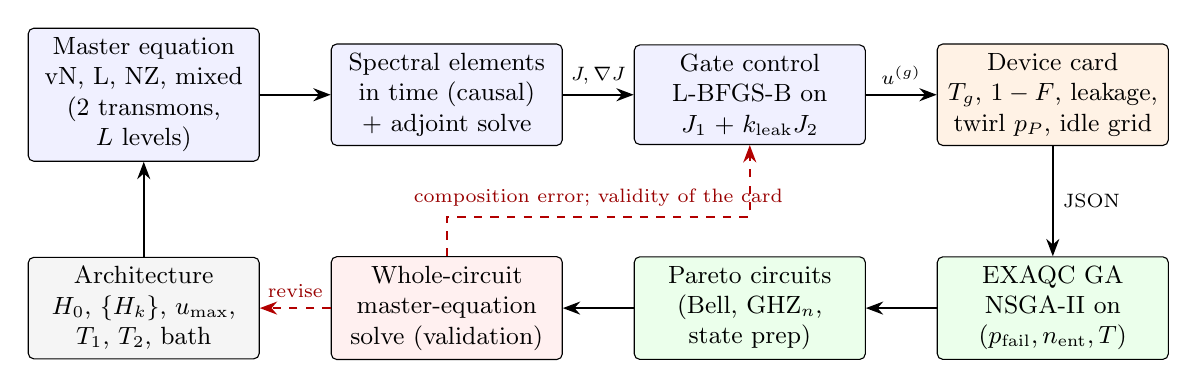
\begin{tikzpicture}[
  node distance=5mm and 9mm,
  box/.style={draw, rounded corners=2pt, align=center, minimum height=11mm,
              text width=27mm, font=\small, fill=#1},
  box/.default={white},
  arr/.style={-{Stealth[length=2.2mm]}, thick},
  lab/.style={font=\scriptsize, align=center}]
  \node[box=blue!6]   (me)   {Master equation\\vN, L, NZ, mixed\\(2 transmons, $L$ levels)};
  \node[box=blue!6, right=of me]  (sem)  {Spectral elements\\in time (causal)\\+ adjoint solve};
  \node[box=blue!6, right=of sem] (oc)   {Gate control\\L-BFGS-B on\\$J_1 + k_{\mathrm{leak}}J_2$};
  \node[box=orange!10, right=of oc] (card) {Device card\\$T_g$, $1-F$, leakage,\\twirl $p_P$, idle grid};
  \node[box=green!8, below=14mm of card] (ga) {EXAQC GA\\NSGA-II on\\$(\pfail, n_{\mathrm{ent}}, T)$};
  \node[box=green!8, left=of ga] (circ) {Pareto circuits\\(Bell, GHZ$_n$,\\state prep)};
  \node[box=red!6, left=of circ] (val) {Whole-circuit\\master-equation\\solve (validation)};
  \node[box=gray!8, left=of val] (arch) {Architecture\\$H_0$, $\{H_k\}$, $u_{\max}$,\\$T_1$, $T_2$, bath};
  \draw[arr] (me) -- (sem);
  \draw[arr] (sem) -- node[lab, above]{$J,\nabla J$} (oc);
  \draw[arr] (oc) -- node[lab, above]{$u^{(g)}$} (card);
  \draw[arr] (card) -- node[lab, right]{JSON} (ga);
  \draw[arr] (ga) -- (circ);
  \draw[arr] (circ) -- (val);
  \draw[arr] (arch) -- (me);
  \draw[arr, dashed, red!70!black] (val.north) -- ++(0,5mm) -| (oc.south)
     node[lab, pos=0.25, above, text=red!60!black]{composition error; validity of the card};
  \draw[arr, dashed, red!70!black] (val.west) -- node[lab, above, text=red!60!black]{revise} (arch.east);
\end{tikzpicture}
\caption{The pipeline. Stage one (blue, orange) computes how to drive each gate
of a universal set on a modelled architecture and reduces the result to a
device card. Stage two (green) searches for circuits against the card. The
dashed paths are the validation loop: whole-circuit solves measure what the
card's per-gate abstraction misses and feed back into the choice of gate
calibration and, if necessary, of the device itself.}
\label{fig:pipeline}
\end{figure}

The reason to build all of this, rather than to take vendor error rates and a
depolarizing model, is a control experiment that we report in
Section~\ref{sec:results}. With the search algorithm, the gate set and the
genome budget held fixed, we ran the search three times, once with no noise
model, once with uniform depolarizing noise at the true average rates, and once
with the simulated card, and evaluated every resulting circuit under the
simulated card as the common yardstick. The loss from not simulating the
device is monotone in how much physics the search is told, and it is largest
under the non-Markovian model, which a uniform error rate cannot represent at
all. We note that this argument does not depend on the search beating every
hand-built circuit, and in several cases it does not; it depends only on the
observation that the same algorithm returns better circuits when it is given a
better description of the device.

The remainder of the report is organized as follows.
Section~\ref{sec:models} fixes the device and the four environment models.
Section~\ref{sec:sem} describes the spectral-element solver and why its
resolution must grow with the number of transmon levels.
Section~\ref{sec:oc} describes the control problem and its adjoint gradient,
including the leakage functional. Section~\ref{sec:cards} describes the
construction of the device card. Section~\ref{sec:ga} describes the circuit
search. Section~\ref{sec:results} reports results to date,
Section~\ref{sec:compute} the compute plan, and Section~\ref{sec:open} the
open problems.

\section{The device and the environment models}
\label{sec:models}

Each qubit is a transmon truncated to $L$ levels, with the Duffing Hamiltonian
$H_j = \Delta_j a_j^\dagger a_j - (\alpha/2)\, a_j^\dagger a_j^\dagger a_j a_j$
in the frame rotating at the frequency of transmon~1, so that $\Delta_1 = 0$
and $\Delta_2 = \delta_{2q}$ is the detuning of the second transmon. Each
transmon carries two drives, $H_x = (a + a^\dagger)/2$ and
$H_y = i(a^\dagger - a)/2$, with piecewise-constant amplitudes bounded by
$|u| \le u_{\max}$, so the two-qubit problem has four controls. The two
transmons are coupled by a static exchange term
$g(a_1^\dagger a_2 + a_1 a_2^\dagger)$. Throughout, $\alpha/2\pi = 200$~MHz,
$g/2\pi = 5$~MHz, $T_1 = 100\,\mu$s and $T_2 = 60\,\mu$s; single-qubit gates
last 50~ns and the CNOT 200~ns. The cards in use today were computed at
$\delta_{2q}/2\pi = 300$~MHz, a value we now know to be a poor choice, for the
reason given in Section~\ref{sec:collision}.

The levels above $|1\rangle$ matter for two reasons. They are where population
goes when a pulse is fast or strong (leakage), and their presence shifts the
energies of the computational states. A model with $L = 2$ cannot leak and
therefore cannot be trusted to say how fast a gate may be; a model with too few
levels misrepresents the levels into which population leaks, which is
worse, because the optimizer can then exploit the truncation. We return to
this in Section~\ref{sec:collision}.

We work with four models of the environment, in increasing order of realism.
Writing $x(t) = \vecop(\rho(t))$ for the column-stacked density matrix of the
system, each model is a linear equation for $x$:
\begin{align}
  \text{(vN)}\quad & \dot x = A_{\mathrm H}(t)\, x, \label{eq:vn}\\
  \text{(L)}\quad  & \dot x = A_0(t)\, x, \label{eq:lind}\\
  \text{(NZ)}\quad & \dot x = A_{\mathrm H}(t)\, x
       + \int_0^t K(t-s)\, x(s)\, \dd s, \label{eq:nz}\\
  \text{(M)}\quad  & \dot x = A_0(t)\, x
       + \int_0^t K(t-s)\, x(s)\, \dd s. \label{eq:mixed}
\end{align}
Here $A_{\mathrm H}$ is the matrix of the commutator $-i[H(t),\cdot\,]$ and
$A_0 = A_{\mathrm H} + \sum_k \mathcal D[L_k]$ adds Lindblad dissipators with
jump operators $L_- = T_1^{-1/2} a$ and $L_\phi = (2\gamma_\phi)^{1/2} a^\dagger a$
on each transmon, $\gamma_\phi = 1/T_2 - 1/(2T_1)$. In the code these four
models are called \texttt{schrod}, \texttt{lindblad\_markov},
\texttt{lindblad\_nm} and \texttt{mixed}; we use those names in the tables.
We note that \texttt{schrod} is solved as the closed-system superoperator
equation, so all four models share one solver.

The memory kernel describes dephasing by a bath whose correlations decay on a
time scale comparable to the gate. We take $K(\tau) = -C(\tau)\, S$, where
$S\rho = [\sigma_z,[\sigma_z,\rho]]$ is the double commutator with the
computational $\sigma_z$ and
\begin{equation}
  C(\tau) = A\, e^{-\gamma\tau} \cos(\Omega\tau).
  \label{eq:kernel}
\end{equation}
Equation~\eqref{eq:nz} is a Volterra integro-differential equation, a
Nakajima--Zwanzig equation, and it is non-local in time: the rate of change of
the state depends on its whole history. For $\Omega = 0$ the kernel is a single
Lorentzian, and the same physics can be represented by adjoining one damped
harmonic mode (a pseudomode) to each transmon, coupled to $\sigma_z$ and
decaying at rate $\kappa$, which makes the generator time-local at the price of
a larger Hilbert space \cite{Tamascelli2018}. The two descriptions agree when
$\gamma = \kappa/2$ and $A = g_{\mathrm{pm}}^2$ with
$g_{\mathrm{pm}} = (\gamma_\phi\kappa/8)^{1/2}$, which fixes the bath so that
its white-noise limit reproduces the Markovian $\gamma_\phi$. We use a memory
time $1/\kappa = 50$~ns, equal to the single-qubit gate time. The first card
set was built with the pseudomode description, truncated to $K_{\mathrm{aux}} = 2$
Fock levels per mode; the spectral solver integrates the kernel directly and
needs no such truncation, and it also covers $\Omega > 0$, a damped-oscillatory
kernel that no single pseudomode realizes.

The memory kernel changes the qualitative behaviour of an idle qubit. Under
the Markovian model the coherence of an idle qubit decays exponentially from
the first instant. Under the kernel~\eqref{eq:kernel} the decay is quadratic in
time for $t \ll 1/\gamma$, and a qubit that is being driven averages part of
the slow noise away, much as a dynamical-decoupling sequence would. A circuit
search that sees this difference can exploit it, and one that sees only a
single error rate per gate cannot. That is the physical content behind the
control experiment described in the introduction.

\section{Spectral elements in time}
\label{sec:sem}

In this section we describe the solver. A fuller treatment, with convergence
theory and benchmarks against time-stepping methods, is in the companion
manuscript \cite{VogtSISC}, whose summary is that the order of a time-stepping
scheme sets floors on the accuracy of both the reported objective and the
control the optimizer returns, and that high-order collocation clears them.

\subsection{Collocation on one element}

Let $\{t_j\}_{j=0}^N$ be Chebyshev--Gauss--Lobatto nodes on an interval and
$\ell_k$ the Lagrange polynomials on those nodes. We seek a degree-$N$
polynomial $x_N(t) = \sum_k \ell_k(t)\, x_k$ that satisfies the initial
condition at $t_0$ and the equation at the remaining nodes,
\begin{equation}
  \sum_{k=0}^N D_{jk}\, x_k = A(t_j)\, x_j + \sum_{k=0}^N W_{jk}\, x_k,
  \qquad j = 1,\dots,N,
  \label{eq:colloc}
\end{equation}
where $D$ is the spectral differentiation matrix and
$W_{jk} = \int_0^{t_j} K(t_j - s)\, \ell_k(s)\, \dd s$ are Volterra blocks,
computed by Gauss--Legendre quadrature with $2N + 16$ points against the
interpolant. Equations without memory simply omit $W$. For analytic data the
error decays geometrically in $N$, which is the property that distinguishes the
method from Euler or trapezoidal stepping, whose errors decay algebraically.

\subsection{Elements and the causal solve}

The controls are piecewise constant on $M$ segments, so the solution has a
corner at every segment boundary and a single global polynomial would converge
only algebraically. The classical remedy is the spectral element method
\cite{Patera1984}: one element per control segment, $N{+}1$ nodes on each, and
continuity of the state across the interfaces. The memory integral at a node of
element $m$ splits exactly into a sum over all earlier elements plus a partial
integral over element $m$ itself, and each piece is integrated with the same
quadrature, so the memory term keeps its spectral accuracy element by element.

Assembled naively this is one dense linear system of side $M(N{+}1)d^2$, with
$d = L^n$ the Hilbert-space dimension for $n$ transmons. That is affordable for
one qubit and not for two: on the grids in use when the causal solver was
written, the dense operator needed about 97~GB at four levels per transmon and
578~GB at five. However, the operator is
block-lower-triangular in the element index, because the memory integral looks
only backwards. Element $m$ couples to its own nodes, to the last node of
element $m-1$ through the continuity row, and to the history of elements
$m' < m$. The system can therefore be solved by forward substitution, one
element at a time, as sketched in Figure~\ref{fig:causal}. The only dense
factorization is of one element block of side $B = (N{+}1)d^2$, and the
history of earlier elements enters the right-hand side. The discretization is
unchanged, so the answer and the convergence rate are unchanged; the causal
solve reproduces the dense assembly to roundoff. The transposed system that
the gradient requires is block-upper-triangular and is solved by backward
substitution over the same factors. The arithmetic cost is
$O(M^2 B^2 + M B^3)$, the $M^2$ term coming from the history, the direct
analogue of the $O(n^2)$ history sum of a time stepper but with spectral
accuracy per element.

\begin{figure}[htbp]
\centering
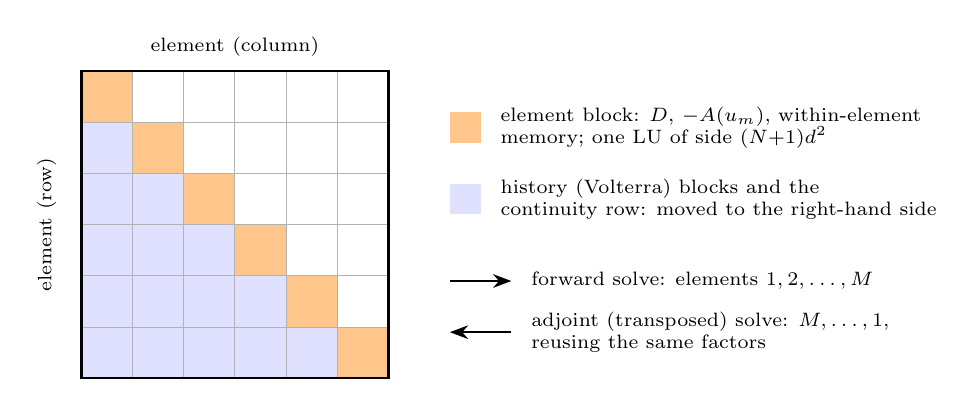
\begin{tikzpicture}[x=6.5mm, y=6.5mm, font=\scriptsize]
  % block lower-triangular matrix, 6 elements
  \foreach \i in {0,...,5} {
    \foreach \j in {0,...,5} {
      \pgfmathtruncatemacro{\r}{5-\i}
      \ifnum\j<\i
        \fill[blue!12] (\j,\r) rectangle ++(1,1);
      \fi
      \ifnum\j=\i
        \fill[orange!45] (\j,\r) rectangle ++(1,1);
      \fi
    }
  }
  \draw[step=1, gray!60] (0,0) grid (6,6);
  \draw[thick] (0,0) rectangle (6,6);
  \node[above] at (3,6.1) {element (column)};
  \node[rotate=90, above] at (-0.3,3) {element (row)};
  % legend
  \fill[orange!45] (7.2,4.6) rectangle ++(0.6,0.6);
  \node[right, align=left] at (8,4.9) {element block: $D$, $-A(u_m)$, within-element\\memory; one LU of side $(N{+}1)d^2$};
  \fill[blue!12] (7.2,3.2) rectangle ++(0.6,0.6);
  \node[right, align=left] at (8,3.5) {history (Volterra) blocks and the\\continuity row: moved to the right-hand side};
  \draw[-{Stealth}, thick] (7.2,1.9) -- ++(1.2,0);
  \node[right, align=left] at (8.6,1.9) {forward solve: elements $1, 2, \dots, M$};
  \draw[{Stealth}-, thick] (7.2,0.9) -- ++(1.2,0);
  \node[right, align=left] at (8.6,0.9) {adjoint (transposed) solve: $M, \dots, 1$,\\reusing the same factors};
\end{tikzpicture}
\caption{Block structure of the spectral-element system. Causality makes it
block-lower-triangular, so it is solved one element at a time and the largest
dense object is a single element block.}
\label{fig:causal}
\end{figure}

\subsection{Resolution must scale with the number of levels}

The anharmonic ladder raises the top frequency of the generator as levels are
added, and the elements must resolve it. Table~\ref{tab:freq} lists the largest
imaginary part of the eigenvalues of the two-transmon generator and the number
of oscillation cycles that fit in a 2.5~ns segment. Our first two-qubit
campaign used $M = 8$ segments over 200~ns, that is, 25~ns elements carrying
more than forty oscillations each at five levels; it never converged in $N$
(the infidelity moved erratically, $9.4\times10^{-4}$ at $N = 24$), and eight
CNOT cells returned $1 - F \approx 0.68$--$0.70$ after about seven hours each.
The cause was the grid, not the optimizer, and the diagnostic was available in
the output before the cause was understood: on the memoryless models, where the
per-segment matrix-exponential propagator is exact, the spectral and exact
objectives disagreed by about $0.1$ on the CNOT runs while agreeing to five
digits on every single-qubit run. A large gap between the two on a memoryless
model indicates an unresolved grid.

\begin{table}[htbp]
\centering
\caption{Top frequency of the two-transmon generator against the number of
levels per transmon, and the grids validated against the exact propagator on
the memoryless model (agreement $|J_{\mathrm{SEM}} - J_{\mathrm{exact}}|$ at a
fixed control). The block is the side of one element system, $(N{+}1)d^2$.}
\label{tab:freq}
\small
\begin{tabular}{ccc@{\qquad}cccc}
\toprule
levels & $\max|\mathrm{Im}\,\lambda(A)|$ (rad/ns) & cycles per 2.5~ns
  & $M$ & $N$ & block & $|J_{\mathrm{SEM}} - J_{\mathrm{exact}}|$ \\
\midrule
3 & 3.84  & 1.5 & -- & -- & -- & -- \\
4 & 6.41  & 2.5 & 80 & 20 & 5376  & $6.99\times10^{-9}$ \\
5 & 10.19 & 4.1 & 80 & 20 & 13125 & $5.69\times10^{-7}$ \\
\bottomrule
\end{tabular}
\end{table}

Both validated grids sit far below the gate infidelities of interest. We note
that coarser elements with more nodes do not substitute: $M = 160$, $N = 8$ at
five levels gives a gap of $2.31\times10^{-3}$. Since resampling a pulse onto a
different $M$ changes the pulse, a convergence study must fix $M$ and vary only
$N$.

\section{Gate-level optimal control with leakage}
\label{sec:oc}

\subsection{The control problem}

For each gate $g$ of the universal set $\{H, X, Z, S, T, \mathrm{CNOT}\}$ and
each environment model we solve
\begin{equation}
  \min_{|u| \le u_{\max}} \; J_1(u) + k_{\mathrm{leak}}\, J_2(u)
     + k_{\mathrm{top}}\, J_{\mathrm{top}}(u) + \beta \langle u^2 \rangle .
  \label{eq:ocp}
\end{equation}
The first term is the gate infidelity on the computational subspace.
Writing $X(T)$ for the solution whose columns are the images of the $\dc^2$
embedded computational basis operators $|i\rangle\langle j|$, and $Y$ for the
corresponding target, the code minimizes $J_1 = 1 - \mathrm{Re}\langle Y,
X(T)\rangle/\dc^2$ and reports the average gate infidelity
$1 - (\dc F_e + 1)/(\dc + 1)$ with $F_e = 1 - J_1$. Because $X(T)$ is
projected onto the computational subspace before the comparison, an arbitrary
rotation of the leakage levels is not charged as infidelity, which is the
correct convention for a gate that is only ever asked to act on qubits. The
second term is the time-averaged leakage,
\begin{equation}
  J_2 = \frac{1}{T}\int_0^T \Big(1 - \mathrm{Tr}\big[\Pcomp\, \rho(t)\big]\Big)\, \dd t,
  \qquad \rho(0) = \Pcomp/\dc,
  \label{eq:leak}
\end{equation}
the population outside the computational subspace when the gate acts on the
maximally mixed computational state, integrated by the trapezoid rule on the
collocation nodes. The third term, used only in the most recent CNOT run, is a
penalty with weight $k_{\mathrm{top}}$ on population in the highest retained
level, introduced because $J_2$ alone did not keep that level empty
(Section~\ref{sec:cnotstatus}). The last term is a small amplitude regularizer,
$\beta = 10^{-3}$. We minimize~\eqref{eq:ocp} by L-BFGS-B \cite{Byrd1995} with
box constraints on the amplitudes, from several random starts, keeping the
best; this is GRAPE \cite{Khaneja2005} with a quasi-Newton optimizer and a
spectral rather than a piecewise-exponential propagator.

\subsection{The adjoint gradient}

The discrete map from controls to objective is one block-triangular linear
solve, $\mathcal A(u)\, X = b$, followed by smooth algebra, so its exact
gradient comes from one transposed solve with the same factors. For a
functional $\varphi(X)$, let $G = \partial\varphi/\partial \bar X$ and solve
$\mathcal A(u)^\dagger \Lambda = G$. Since $\partial \mathcal A/\partial
u_{m,k} = -B_k$ on the collocation rows of element $m$ and is zero elsewhere,
with $B_k$ the superoperator of control $k$,
\begin{equation}
  \frac{\partial \varphi}{\partial u_{m,k}}
   = \mathrm{Re}\, \Lambda^\dagger B_k^{(m)} X ,
  \label{eq:grad}
\end{equation}
up to the normalization of $\varphi$. The cost of the gradient is therefore
that of one more solve, independent of the number of control parameters,
whereas a central-difference gradient would need two solves per parameter
($4M = 320$ parameters for the CNOT at $M = 80$). For the infidelity $J_1$ the
source $G$ is nonzero only in the rows of the terminal node. The leakage
functional~\eqref{eq:leak} is linear in $X$ at every node, so it rides the same
adjoint, and only the source changes: $G$ is now nonzero at every node, carrying
the trapezoid weight of that node. One forward solve per objective evaluation
is cached and shared by both functionals.

The first version of the code added $k_{\mathrm{leak}} J_2$ to the cost but
supplied only the gradient of $J_1$; the inconsistent gradient broke the Wolfe
line search, and both early runs stopped at exactly twelve iterations with peak
leakage still between 16\% and 40\%. With the leakage gradient in place the
analytic gradient agrees with central differences to $1.4\times10^{-8}$ (one transmon, four levels),
$5.9\times10^{-9}$ (one transmon, five levels) and $1.5\times10^{-8}$ (two
transmons, three levels). We note also a sign subtlety that is easy to get
wrong: because $\partial\mathcal A/\partial u$ carries a minus sign, the leakage
source enters the adjoint without one, and getting it backwards produces a
gradient of the right magnitude and the wrong sign (a relative error of exactly
two).

\section{Device cards}
\label{sec:cards}

The card is the interface between the two stages, and it is deliberately a
plain JSON file: the control code and the circuit code run in different Python
environments and share no process. For each gate the card records the pulse
duration $T_g$, the average gate infidelity, the time-averaged leakage, the
trace lost from the computational subspace, and a Pauli-twirled error channel;
it also records a single-qubit idle channel on a grid of durations.

The channel comes directly from the spectral solve. The solver returns $X(T)$
of shape $d^2 \times \dc^2$, the image of each embedded computational basis
operator, and the embedding is the isometry $W = \bar P \otimes P$ with $P$ the
$d \times \dc$ inclusion of the computational subspace. The restricted channel
is therefore $V_{\mathrm c} = W^\dagger X(T)$, a $\dc^2 \times \dc^2$ matrix,
with no second solve. Let $R_V$ be its Pauli transfer matrix (PTM), the matrix
of the channel in the normalized Pauli basis, and $R_U$ that of the target
unitary. The error channel is $\mathcal E = \mathcal V_{\mathrm c} \circ
\mathcal U^\dagger$, with PTM $R_E = R_V R_U^{\mathsf T}$, and its Pauli twirl
\cite{Wallman2016} has probabilities
\begin{equation}
  p_P = \frac{1}{\dc^2} \sum_Q \chi(P,Q)\, [R_E]_{QQ},
  \qquad \chi(P,Q) = \pm 1
  \label{eq:twirl}
\end{equation}
according to whether the Pauli strings $P$ and $Q$ commute. For a gate that
leaks, $\mathcal V_{\mathrm c}$ is not trace preserving, and the probabilities
sum to the surviving trace, $\sum_P p_P = [R_V]_{II} = 1 - \text{trace loss}$,
rather than to one. What leaks out of the subspace is exactly what is missing
from the sum, and the card builder checks the sum against that quantity rather
than against unity (for the five-level Hadamard,
$1 - 8.552\times10^{-6} = 0.9999915$, as it should be). The no-error
probability $p_{I\cdots I}$ is the card's notion of success, and
$\varepsilon_g = 1 - p_{I\cdots I}$ is the gate's error probability.

Three properties of the card should be kept in view. First, the twirl
discards the coherent part of the control error, so the circuit search cannot
exploit coherent cancellation between gates. Second, the circuit simulator
works with qubits, so it renormalizes the twirl probabilities and the trace
loss disappears from the tier-one simulation; the tier-zero failure
probability, which uses $1 - p_{I\cdots I}$ directly, keeps it and is the more
conservative of the two. Third, a single-qubit gate on a coupled device acts
on two qubits, and reducing its two-qubit twirl to a one-qubit channel on the
driven wire discards the terms that act nontrivially on the spectator. The card
records the discarded mass as \texttt{spectator\_weight}. That number turns out
to be the validity criterion for the whole construction
(Section~\ref{sec:validity}).

The idle channel is the zero-control solution of the same model on a grid of
durations, 50~ns to 1200~ns in 50~ns steps. Consumers interpolate the PTM
diagonal log-linearly between grid points. An earlier version stored one 50~ns
window and extrapolated by a power law, which is exact only for a Markovian
Pauli channel; under the memory kernel the short-time decay is quadratic and
that extrapolation understated a 100~ns idle by a factor of 1.73. The spectral
cards at present carry an idle grid copied from the pseudomode cards, recorded
as such in the card's conventions field, because no spectral idle channel has
yet been computed.

\section{Circuit learning with EXAQC}
\label{sec:ga}

In this section we describe the circuit side in the terms in which it was
built. EXAQC represents a circuit as a genome: a list of gates, each with a
method name, a qubit assignment, a depth coordinate that orders it in the
circuit, an enabled flag and an innovation number. Mutations add, disable,
enable, reorder and qubit-swap gates, and crossover recombines parents. The
device-card plugin adds a noise model, a set of hardware objectives and a
multi-objective population strategy, and changes the framework itself in only
two places, both backward compatible.

\subsection{Noise hooks}

The noise model is told about the circuit as it is built, through four hooks.
At \texttt{begin\_circuit} it computes an as-soon-as-possible schedule of the
enabled gates from the card's durations, which fixes when each wire is busy
and when it idles. At \texttt{before\_gate} it charges each of the gate's wires
for the interval it has spent idle since it was last busy, applying the card's
idle channel for that interval. At \texttt{after\_gate} it applies the gate's
own twirled channel as a set of Kraus operators $\sqrt{p_P}\,P$. At
\texttt{before\_measurement} it charges the terminal idle interval of each
wire. The placement of the idle channel matters more than one might expect.
Pauli channels commute with one another but not with the intervening gates, so
an earlier version that accumulated idle time per wire and applied it at the
end charged a wire idling in $|0\rangle$ before its entangler, which is
harmless, as if it had idled while entangled, which is not. That error
overstated the textbook circuits, which have the longest pre-entangler idle
periods, and it inflated our first headline result.

\subsection{Objectives and selection}

Given a card, the hardware objectives are pure functions of the genome and
need no simulation: the failure probability
\begin{equation}
  \pfail = 1 - \prod_g (1 - \varepsilon_g) \prod_w (1 - \varepsilon^{\mathrm{idle}}_w),
  \label{eq:objectives}
\end{equation}
the number of entanglers $n_{\mathrm{ent}}$, and the makespan
$T_{\mathrm{circ}}$ of the schedule in nanoseconds.
The failure probability $\pfail$ is the tier-zero estimate, the probability
that at least one Pauli error occurs, idle periods included;
$1/(1 - \pfail)$ is the expected number of shots per error-free run. The
duration is depth measured in nanoseconds, which is the quantity that competes
with $T_2$. The task enters as a constraint rather than an objective: for
state preparation we compute the noiseless output, trace out any helper wires,
and require $1 - \langle\psi|\rho|\psi\rangle \le 10^{-3}$, with a penalty on
population parked outside $|0\rangle$ on helper wires. Targets include the four
Bell states and GHZ$_n$ for $n$ up to 12. Keeping the task as a constraint keeps
the front three-dimensional and interpretable: it is the hardware trade-off
among circuits that do the job.

Selection is a steady-state NSGA-II \cite{Deb2002}: non-dominated sorting with
crowding distance, insertion of each child into an archive of fixed size,
removal of the worst genome by (rank, crowding), and binary tournaments for
parents. Infeasible genomes rank after every feasible one, ordered by
constraint violation, so the search may approach the feasible set from
outside. Feasible genomes whose objective vector duplicates an incumbent's are
rejected. We note that an earlier version also rejected infeasible duplicates,
which starves the search whenever the objectives are degenerate, as they are
under a noiseless model; the naive baselines could then never find a feasible
circuit.

\subsection{The procedure and its tiers}

We do not search from nothing. A target state almost always comes with a
decomposition that is exact in the closed system, the textbook circuit, and
that decomposition is the right starting point and the wrong stopping point.
The search seeds its population from it, evaluates candidates by
\eqref{eq:objectives}, requires exact closed-system preparation, improves the
population by NSGA-II, prunes greedily any gate whose removal preserves exact
preparation, and finally adjudicates the front by a density-matrix simulation
with every card channel applied (tier one), not by $\pfail$. The last step is
needed because $\pfail$ is blind to the state: it charges for a $Z$ error on a
wire that holds $|0\rangle$, which costs nothing, and we have observed it
inverting the ranking of two circuits. Seeding matters for a further reason: a
from-scratch search conflates the question of whether hardware conditioning
improves a circuit with the question of whether random mutation can find a
feasible GHZ$_8$ circuit at all, and at that size the second question dominates.
Above tier one sits tier two, the whole circuit solved as one master-equation
problem with the bath carried across gate boundaries, which is the reference
against which the card itself is judged.

One defect in the framework found on the way is worth passing upstream:
\texttt{CircuitGenome.copy()} shared gate objects with the parent, while the
disable, enable, reorder and qubit-swap mutations act in place, so every
mutation rewrote its own parent in the archive. The fix is one call to
\texttt{gate.copy()}, and it affects any run of the framework that keeps
parents.

\section{Results to date}
\label{sec:results}

In this section we report what has been established, in the order in which it
bears on the next decisions. We state at the outset the caveat that governs
everything below: every two-qubit number from the first, resonant device must
be regenerated, and the two-qubit cards on the detuned device are themselves
affected by a frequency collision described in Section~\ref{sec:collision}.
The methodology, the ablation, the cross-evaluation and the naive-versus-%
simulated argument survive; the absolute infidelities do not.

\subsection{Single-qubit spectral cards}

The single-qubit spectral cards are complete at five levels, with all eighty
seeds converged. Table~\ref{tab:1q} lists the best infidelity per gate and
model. Terminal leakage lies between $7\times10^{-6}$ and $3\times10^{-5}$.
Raising the iteration limit from 400 to 2000 changed the best values only in
the fifth digit. The pattern across models is the expected one: under the
Markovian models every gate sits near the decoherence floor of a 50~ns window,
about $3.7\times10^{-4}$ to $4.1\times10^{-4}$, while under the non-Markovian
model the same gates reach $3\times10^{-5}$ to $4\times10^{-5}$, because the
optimizer shapes the pulse to refocus the slow part of the noise. We note that
these are calibrations of an isolated transmon, which is the right calibration
for a tunable-coupler device and the wrong one for a device with fixed
coupling (Section~\ref{sec:validity}).

\begin{table}[htbp]
\centering
\caption{Single-qubit spectral cards: best $1 - F$ (average gate infidelity
from the spectral solve) per gate and model, five levels, 50~ns.}
\label{tab:1q}
\small
\begin{tabular}{lcccc}
\toprule
gate & \texttt{schrod} & \texttt{lindblad\_nm} & \texttt{lindblad\_markov} & \texttt{mixed} \\
\midrule
$X$ & $4.638\times10^{-6}$ & $3.299\times10^{-5}$ & $3.668\times10^{-4}$ & $3.951\times10^{-4}$ \\
$H$ & $6.101\times10^{-6}$ & $3.046\times10^{-5}$ & $3.690\times10^{-4}$ & $3.933\times10^{-4}$ \\
$Z$ & $1.327\times10^{-5}$ & $2.896\times10^{-5}$ & $3.779\times10^{-4}$ & $3.936\times10^{-4}$ \\
$S$ & $2.064\times10^{-5}$ & $3.781\times10^{-5}$ & $3.862\times10^{-4}$ & $4.034\times10^{-4}$ \\
$T$ & $2.040\times10^{-5}$ & $4.092\times10^{-5}$ & $3.862\times10^{-4}$ & $4.067\times10^{-4}$ \\
\bottomrule
\end{tabular}
\end{table}

\subsection{The four-level spectral CNOT}
\label{sec:cnotstatus}

The two-qubit CNOT has been run at four levels per transmon on the validated
grid ($M = 80$, $N = 20$, $T = 200$~ns), under all four models with two seeds
each. Table~\ref{tab:cnot} summarizes the two most recent runs, verified on
20 October 2026. The first continued the leakage-penalized problem to 1200
L-BFGS iterations with $k_{\mathrm{leak}} = 1$; the second replaced the leakage
term by the top-level penalty, $k_{\mathrm{top}} = 10$ and
$k_{\mathrm{leak}} = 0$, for 800 iterations. No cell reports convergence. On
the memoryless models the spectral objective and the exact propagator agree to
about $10^{-9}$, so the numbers are resolved; they are simply not good.

\begin{table}[htbp]
\centering
\caption{Spectral CNOT at four levels per transmon, $M = 80$, $N = 20$,
$T = 200$~ns: best $1 - F$ of two seeds. Peak populations refer to transmon~2.
No cell is flagged converged. Preliminary.}
\label{tab:cnot}
\small
\begin{tabular}{lcc}
\toprule
 & $k_{\mathrm{leak}} = 1$, 1200 it. & $k_{\mathrm{top}} = 10$, $k_{\mathrm{leak}} = 0$, 800 it. \\
\midrule
\texttt{schrod}          & $2.1\times10^{-3}$ & $4.2\times10^{-3}$ \\
\texttt{lindblad\_nm}    & $2.0\times10^{-3}$ & $4.4\times10^{-3}$ \\
\texttt{lindblad\_markov}& $6.0\times10^{-3}$ & $8.6\times10^{-3}$ \\
\texttt{mixed}           & $6.5\times10^{-3}$ & $8.8\times10^{-3}$ \\
\midrule
peak population of $|3\rangle$ & 24--31\% & 3--13\% \\
peak population of $|2\rangle$ & -- & $\approx 48\%$ \\
terminal leakage & $< 10^{-3}$ & $< 10^{-3}$ \\
\bottomrule
\end{tabular}
\end{table}

The populations tell the story. With the leakage penalty, the optimal pulses
route between a quarter and a third of the population of transmon~2 through
its top retained level $|3\rangle$ and bring it back by the end of the gate.
The top-level penalty empties $|3\rangle$ to a few percent, but the optimizer
then routes up to about half the population through $|2\rangle$ instead, and
the infidelity roughly doubles. In both cases the terminal leakage is below
$10^{-3}$, so a card built from either run would look clean, and in both cases
the pulse depends on dynamics in levels that a four-level model represents
poorly. We conclude that four levels are truncation-limited for this gate on
this device, and that the four-level CNOT card is not yet trustworthy as input
to the circuit search. The five-level run, which is the physically preferred
one, was killed for lack of memory at 400~GB: at five levels each element block
has side 13125, each cached LU factor occupies about 2.8~GB, and the solver
keeps all eighty factors for the adjoint pass.

\subsection{A frequency collision in the device}
\label{sec:collision}

A separate line of work on the same device, a GRAPE-only study at three
levels, found the cause of the excursions in Table~\ref{tab:cnot}. In the frame
of transmon~1 the levels of transmon~2 lie at
$E_n = n\,\delta_{2q} - (\alpha/2)\, n(n-1)$, which for
$\delta_{2q}/2\pi = 300$~MHz and $\alpha/2\pi = 200$~MHz gives 0, 300, 400,
300 and 0~MHz for $n = 0,\dots,4$. The states $|1\rangle$ and $|3\rangle$ of
transmon~2 are degenerate, because $2\delta_{2q} = 3\alpha$, and so are
$|0\rangle$ and $|4\rangle$. A pulse with spectral content near $\pm 100$~MHz
then drives $|1\rangle \to |3\rangle$ through a barely populated $|2\rangle$.
A plain propagation, independent of every solver used here, reproduces the
effect, with a level-three population of 44\% at four levels and 51\% at five
to six levels, converged at five. Neither a larger leakage weight
($k_{\mathrm{leak}} = 100$) nor a weaker drive removes it. At
$\delta_{2q}/2\pi = 150$~MHz and $u_{\max} = 0.3$~rad/ns, by contrast,
four-level CNOT designs re-scored at five levels hold their infidelity
($5\times10^{-5}$ designed, $1.0\times10^{-4}$ and $4.7\times10^{-5}$ re-scored
for two seeds), and that is the only setting tested in which the CNOT
truncation converges. The default detuning therefore sits on a collision, and
every stored two-qubit card on the detuned device is affected, both the
pseudomode GRAPE cards and the spectral runs of Table~\ref{tab:cnot}. The
three-level study has already moved to 150~MHz; the CNOT cards of this project
must follow.

\subsection{When the card is valid}
\label{sec:validity}

The most consequential finding so far concerns not a number but the domain of
validity of the card. The first device placed both transmons at the same
frequency, so the always-on exchange was resonant: at $g/2\pi = 5$~MHz the swap
time $\pi/2g$ is 50~ns, exactly the single-qubit gate time, and with no
control at all $|10\rangle$ transfers completely to $|01\rangle$ in 50~ns. An
idle wire on that device does not hold its state, so an idle channel computed
on a lone transmon is qualitatively wrong. A pulse-level solve of a textbook
Bell circuit, with each gate's calibrated pulse laid on the coupled device at
its scheduled time, returned $1 - F = 0.686$.

Detuning the second transmon by 300~MHz removes the resonance, since idling
for 50~ns then preserves $|10\rangle$ to $10^{-16}$, but it does not rescue
the per-wire card. Table~\ref{tab:composition} compares, for one embedded
single-qubit pulse calibrated in isolation, the error the coupled device
actually produces with the error the card predicts. Even off resonance the card
is optimistic by a factor of 588 in the closed system and 10.5 under the
non-Markovian model. Calibrating the single-qubit gates in situ, as targets
$U \otimes I$ on the coupled device, gives honest numbers but reveals a
closed-system floor of about $5\times10^{-4}$ for a 50~ns single-qubit gate,
comparable to the CNOT, and the \texttt{spectator\_weight} field shows that
between 53\% and 95\% of each in-situ single-qubit gate's twirled error acts
on the spectator (on the current detuned cards: 53--78\% under
\texttt{schrod}, 78--88\% under \texttt{lindblad\_markov}, 66--91\% under
\texttt{lindblad\_nm} and 80--95\% under \texttt{mixed}). A per-wire Pauli
channel discards most of that error.

\begin{table}[htbp]
\centering
\caption{Composition error of the per-wire card for an isolated single-qubit
pulse embedded in the coupled device. ``Embedded'' is the error of that pulse
solved on the two-transmon device; ``card'' is the card's entry for it.}
\label{tab:composition}
\small
\begin{tabular}{llccc}
\toprule
$\delta_{2q}/2\pi$ & model & embedded & card & card underestimate \\
\midrule
0~MHz   & \texttt{schrod}       & $6.87\times10^{-1}$ & $3.4\times10^{-7}$ & $2\times10^{6}$ \\
300~MHz & \texttt{schrod}       & $2.00\times10^{-4}$ & $3.4\times10^{-7}$ & 588 \\
300~MHz & \texttt{lindblad\_nm} & $1.88\times10^{-4}$ & $1.8\times10^{-5}$ & 10.5 \\
\bottomrule
\end{tabular}
\end{table}

The resolution is architectural. With a tunable coupler, the exchange is on
only during the entangler and off during single-qubit gates and idling, which
is how current hardware operates. On that architecture the ratio of the
embedded single-qubit error to its card entry is 0.38 in the closed system and
0.94 under the Markovian model, instead of 588. We therefore state the scope of
the method as follows: the per-wire device card is a valid abstraction for
tunable-coupler devices, and \texttt{spectator\_weight} is a computable
criterion that says so; on fixed-coupling devices the card is inadequate, and
the simulation itself measures by how much. We regard this criterion, derived
from the physics rather than assumed, as a more useful contribution than the
headline it replaced.

\subsection{Circuit-level results}

The circuit-level results come in two generations, and we keep them apart.
The first generation used the resonant device. On Bell preparation every card
agreed on the structure, one Hadamard and one CNOT in 250~ns, and under the two
non-Markovian cards the search placed a logically inert $T$ gate on the
spectator wire during the Hadamard, because on those cards a driven qubit
dephased less than an idle one. On GHZ$_3$ and GHZ$_4$ an apparent tenfold
improvement over the textbook cascade did not survive two corrections, the
idle placement of Section~\ref{sec:ga} and the idle grid of
Section~\ref{sec:cards}; after them the textbook fan-out beat every searched
circuit at GHZ$_4$ on every dissipative card. What survived, isolated by
ablation, is a mechanism: in the learned GHZ$_3$ circuit, a chain of phase gates
on wire~1 summing to $2\pi$, collectively an identity, keeps that wire driven
during the 200~ns in which it holds coherence and would otherwise idle. Against
the textbook cascade with the same duration and entangler count, it changes the
infidelity from $1.917\times10^{-5}$ to $2.035\times10^{-5}$ in the closed
system (it hurts), leaves the Markovian card unchanged ($1.1998\times10^{-2}$
against $1.2004\times10^{-2}$), and improves the non-Markovian card from
$8.891\times10^{-4}$ to $2.848\times10^{-4}$, a factor of 3.12. The effect
appears only where the model has memory.

The naive-versus-simulated control experiment also belongs to the first
generation, and Table~\ref{tab:naive} gives its GHZ$_4$ result. The search
algorithm, gate set and budget are identical in every row; only the noise
model the search was given differs, and every circuit is judged by tier one
under the true card. The cost of not simulating is a factor of 4.1, 14.1 and
3.7 for the noiseless search and 1.4, 4.3 and 1.3 for uniform depolarizing,
under the Markovian, non-Markovian and mixed cards respectively. It is
monotone in how much physics the search sees and largest under memory, which a
uniform model cannot express. We note the limit of the claim: the textbook
fan-out still beats every search variant at GHZ$_4$, so the result is that
conditioning recovers most of the gap to the best known circuit, not that the
search wins.

\begin{table}[htbp]
\centering
\caption{GHZ$_4$: tier-one infidelity of the best circuit found by the same
search given different noise models, all judged under the true card (first
generation, resonant device; to be regenerated).}
\label{tab:naive}
\small
\begin{tabular}{lccc}
\toprule
search was given & \texttt{lindblad\_markov} & \texttt{lindblad\_nm} & \texttt{mixed} \\
\midrule
no noise              & $7.75\times10^{-2}$ & $5.63\times10^{-3}$ & $8.35\times10^{-2}$ \\
uniform depolarizing  & $2.68\times10^{-2}$ & $1.73\times10^{-3}$ & $2.91\times10^{-2}$ \\
simulated card        & $2.16\times10^{-2}$ & $7.14\times10^{-4}$ & $2.57\times10^{-2}$ \\
card, then pruned     & $1.91\times10^{-2}$ & $3.98\times10^{-4}$ & $2.24\times10^{-2}$ \\
\bottomrule
\end{tabular}
\end{table}

The second generation uses the detuned device with in-situ single-qubit
calibration, built from pseudomode GRAPE. Table~\ref{tab:standard} gives the
tier-one infidelity of the standard circuits under its four cards. All are
exact in the closed system to $3\times10^{-16}$, and none is error-free even
under \texttt{schrod}, since the in-situ gates carry a crosstalk floor near
$5\times10^{-4}$. On these cards single-qubit gates are no longer nearly free,
so adding gates is expensive, and the Bell searches bear this out: across the
four Bell states and four models, the best learned circuit improves on the
standard one by at most 3\% (for $|\Phi^-\rangle$, an $XH$ preparation in place
of $HZ$), and in half the cells not at all.

\begin{table}[htbp]
\centering
\caption{Standard circuits on the detuned cards (second generation): tier-one
$1-F$. The device sits on the frequency collision of
Section~\ref{sec:collision}, so these numbers are provisional.}
\label{tab:standard}
\small
\begin{tabular}{llccccc}
\toprule
task & circuit & \texttt{schrod} & \texttt{lindblad\_markov} & \texttt{lindblad\_nm} & \texttt{mixed} & $T$ (ns) \\
\midrule
$|\Phi^+\rangle$ & $H_0\,\mathrm{CX}_{01}$          & $3.42\times10^{-4}$ & $5.47\times10^{-3}$ & $5.52\times10^{-4}$ & $5.59\times10^{-3}$ & 250 \\
$|\Phi^-\rangle$ & $H_0 Z_0\,\mathrm{CX}_{01}$      & $6.30\times10^{-4}$ & $6.36\times10^{-3}$ & $8.46\times10^{-4}$ & $6.51\times10^{-3}$ & 300 \\
$|\Psi^+\rangle$ & $X_1 H_0\,\mathrm{CX}_{01}$      & $6.14\times10^{-4}$ & $5.81\times10^{-3}$ & $8.21\times10^{-4}$ & $5.93\times10^{-3}$ & 250 \\
$|\Psi^-\rangle$ & $X_1 H_0 Z_0\,\mathrm{CX}_{01}$  & $9.02\times10^{-4}$ & $6.71\times10^{-3}$ & $1.12\times10^{-3}$ & $6.85\times10^{-3}$ & 300 \\
GHZ$_3$ & cascade = fan-out & $4.03\times10^{-4}$ & $1.37\times10^{-2}$ & $1.50\times10^{-3}$ & $1.46\times10^{-2}$ & 450 \\
GHZ$_4$ & cascade           & $4.65\times10^{-4}$ & $2.49\times10^{-2}$ & $3.54\times10^{-3}$ & $2.76\times10^{-2}$ & 650 \\
GHZ$_4$ & fan-out           & $4.65\times10^{-4}$ & $1.76\times10^{-2}$ & $1.12\times10^{-3}$ & $1.80\times10^{-2}$ & 450 \\
\bottomrule
\end{tabular}
\end{table}

The GHZ$_n$ benchmark on the same cards seeds the search from the textbook
cascade and runs four seeds for each $n$ from 2 to 8 and each card.
Table~\ref{tab:ghzn} gives the result under the non-Markovian card and the
cascade-to-learned ratio under all three dissipative cards. The ratio is one
for $n \le 3$, as predicted, and opens from $n = 4$, because the cascade's
duration grows linearly in $n$ while the fan-out's grows logarithmically.
The table also shows where the gain comes from. Under the Markovian and mixed
cards the learned circuit is the fan-out, to the digits shown, for
$n \le 7$; a search with no noise model finds the same circuit for $n \le 6$,
because it too minimizes duration. Most of the cascade-to-learned gain is
therefore depth reduction, which a compiler pass would also deliver. A gain
specific to the card appears in one cell, $n = 5$ under the non-Markovian card,
where the learned circuit ($2.64\times10^{-3}$, seven gates) beats the fan-out
($3.39\times10^{-3}$) by a factor of 1.29; for $n = 4, 6, 7, 8$ under the same
card the learned circuit is worse than the fan-out (marginally at $n = 6$), and
at $n = 8$ no search variant found the 650~ns fan-out. We note also that the
fan-out infidelity under the non-Markovian card falls from $n = 6$ to $n = 8$
at fixed duration, which we have not yet explained and which should be checked
when the benchmark is rerun. These are second-generation numbers
on a colliding device and must be rerun on corrected cards before they are
quoted.

\begin{table}[htbp]
\centering
\caption{GHZ$_n$ seeded from the cascade (second generation, detuned cards,
four seeds). Columns three to seven: tier-one $1-F$ under
\texttt{lindblad\_nm} for the cascade, the fan-out, and the best circuit
learned against the card, against uniform depolarizing noise, and with no
noise. ``gates'' counts the learned (card) circuit. The last three columns are
cascade over learned (card) under each dissipative card. Provisional.}
\label{tab:ghzn}
\small
\setlength{\tabcolsep}{4pt}
\begin{tabular}{ccccccccccc}
\toprule
 & $T$ (ns) & \multicolumn{5}{c}{\texttt{lindblad\_nm}, $1-F$} & & \multicolumn{3}{c}{cascade / learned} \\
\cmidrule(lr){3-7}\cmidrule(lr){9-11}
$n$ & casc./fan & cascade & fan-out & card & depol. & none & gates & NM & Markov & mixed \\
\midrule
2 & 250/250 & 5.52e-4 & 5.52e-4 & 5.52e-4 & 5.52e-4 & 5.52e-4 & 2 & 1.00 & 1.00 & 1.00 \\
3 & 450/450 & 1.50e-3 & 1.50e-3 & 1.50e-3 & 1.50e-3 & 1.50e-3 & 3 & 1.00 & 1.00 & 1.00 \\
4 & 650/450 & 3.54e-3 & 1.12e-3 & 1.39e-3 & 1.12e-3 & 1.12e-3 & 5 & 2.55 & 1.42 & 1.54 \\
5 & 850/650 & 6.72e-3 & 3.39e-3 & 2.64e-3 & 3.39e-3 & 3.39e-3 & 7 & 2.55 & 1.26 & 1.34 \\
6 & 1050/650 & 1.10e-2 & 3.02e-3 & 3.04e-3 & 3.02e-3 & 3.02e-3 & 9 & 3.63 & 1.57 & 1.73 \\
7 & 1250/650 & 1.64e-2 & 2.64e-3 & 2.91e-3 & 2.64e-3 & 6.20e-3 & 8 & 5.64 & 1.86 & 2.13 \\
8 & 1450/650 & 2.29e-2 & 2.27e-3 & 6.85e-3 & 7.08e-3 & 7.08e-3 & 17 & 3.34 & 1.61 & 1.79 \\
\bottomrule
\end{tabular}
\end{table}

\section{Compute plan and cost}
\label{sec:compute}

In this section we set out the computation that the next step requires and
what is known about its cost. The next step is to re-run the CNOT at
$\delta_{2q}/2\pi = 150$~MHz, at four and at five levels per transmon, under
all four models, on the validated grid $M = 80$, $N = 20$, and to rebuild the
two-qubit cards from the result. The five-level run is the one that matters,
and its obstacle is memory rather than arithmetic. At five levels the element
block has side $B = 13125$; one complex LU factor of that size occupies about
2.8~GB, and the solver keeps all eighty for the adjoint, which is what exhausted
the 400~GB allocation. At four levels the block is 5376 and the eighty factors
fit in about 37~GB. Three remedies are available that leave the discretization
untouched: refactoring each element block during the backward pass instead of
caching it, which doubles the factorization work and bounds the memory by one
block; writing the factors to node-local disk; or moving the element solves to
the GH200 nodes on tigris, which pair a Grace CPU with a GPU of 96~GB. A
benchmark on one GH200 node of tigris (job 382671) measured where the time goes.
On the 72 Grace cores one four-level evaluation takes 105~s under the
closed-system model and 148~s under the memory model. The eighty LU
factorizations account for 43~s of it, and the GPU does the same factorization
in 0.029~s per block instead of 0.59~s. We note that a further 43~s goes to the
gradient contraction, which is written as an unoptimized \texttt{einsum}; recast
as one matrix product per element it falls below a second on either processor.
Block assembly (10--16~s) and the history sums of the memory models (about
40~s) are Python loops that become matrix products in the same way. At five
levels a block factorizes in 4.9~s on the CPU and 0.20~s on the GPU. The
projected GPU figures in Table~\ref{tab:compute} assume these loops are moved
to the device with the factorizations; the eighty five-level factors (220~GB)
exceed the 96~GB of device memory, so they are either kept in the 480~GB of host
memory or recomputed in the backward pass, at about 16~s per evaluation.

% === COMPUTE-TABLE ===
\begin{table}[htbp]
\centering
\caption{Cost of one objective-and-gradient evaluation of the spectral CNOT
($M = 80$, $N = 20$) and of a campaign (four models, two seeds, 1200
iterations, about one evaluation per iteration). Measured on tigris job 382671
except where marked $^\dagger$, which are projections from the measured
factorization times with the Python loops vectorized.}
\label{tab:compute}
\small
\begin{tabular}{lcccc}
\toprule
configuration & block side & factors (GB) & s per evaluation & campaign (node-h) \\
\midrule
4 levels, CPU (72 cores), current code & 5376  & 37  & 105--148 & 280--395 \\
4 levels, GPU (GH200)                  & 5376  & 37  & $\approx 5^\dagger$ & $\approx 13^\dagger$ \\
5 levels, CPU (72 cores)               & 13125 & 220 & $\geq 400^\dagger$ & $\approx 1100^\dagger$ \\
5 levels, GPU (GH200)                  & 13125 & 220 & $\approx 20^\dagger$ & $\approx 55^\dagger$ \\
\bottomrule
\end{tabular}
\end{table}
% === END COMPUTE-TABLE ===

For orientation, the GRAPE code of the three-level study, which uses a
matrix-free action-of-the-exponential propagator rather than collocation, ran
its CNOT gradient on one GH200 between 22 times faster than on four CPU cores
(one sample per gradient) and 193 times faster (sixteen samples batched into
one gradient, four levels, mixed model). The spectral solve differs in that its dominant cost is dense LU
factorization of large blocks, so we do not assume that speedup carries over;
the benchmark above measures it directly, at about twenty times for the factorization itself. Stage two is cheap by comparison: a circuit
evaluation is a product of tabulated numbers plus, for the archive, one small
density-matrix simulation, and the GHZ$_n$ benchmark of
Table~\ref{tab:ghzn}, 168 searches, ran as one CPU array job.

\section{Open problems and next steps}
\label{sec:open}

The first and blocking problem is the two-qubit card. It must be recomputed
off the collision, at five levels, and checked against the same CNOT re-scored
at six before it is fed to the search. Only then do the second-generation
circuit results become quotable, and we expect the comparison of spectral
against pseudomode cards to be informative in itself, provided levels and
leakage weights are matched; a spurious gap of $1.4\times10^{-4}$ was once
reported from exactly that mismatch. We note also that the spectral two-qubit
problem, in the local copy of the code, attaches the memory kernel to $\sigma_z$ of
transmon~1 only, whereas the pseudomode two-qubit problem carries a pseudomode
on each transmon. This should be reconciled before the two card families are
compared, and it may account for part of the closeness of the
\texttt{schrod} and \texttt{lindblad\_nm} entries in Table~\ref{tab:cnot}.

The second problem is the idle channel. The spectral cards borrow the
pseudomode idle grid; an idle-dominated result should not be quoted until the
idle channel is recomputed with the spectral solver, which is a cheap,
zero-control solve.

The third is validation at tier two. The whole-circuit solver lays each gate's
pulse on the device at its scheduled time and integrates the circuit as one
master-equation problem, with no card and with bath memory retained across
gates. It must be extended to segmented generators, with the coupling on only
during the entangler, to model the tunable-coupler architecture for which the
card is valid. It exists for two qubits only, so every GHZ number remains a
surrogate prediction until a three-qubit validator is built.

The fourth concerns the search. The feasible set is connected under gate
addition but not under the single-gate moves EXAQC provides, so a cascade
cannot always become a fan-out without passing through infeasible circuits,
and from-scratch runs converge to feasible local optima that no single
deletion escapes. Seeding and restarts mitigate this. A structure-preserving
move, such as rewiring an entangler or crossover at the level of subcircuits,
would address it directly, and it is the place where the GA expertise of the
collaboration is most likely to change the outcome. The tasks are also small:
state preparation makes entangler count and duration compete, but a
three-objective front over a handful of gates is a weak instrument, and the
variational classifier circuits of the EXAQC line are the natural next target.

The fifth is the card format itself. A Pauli twirl cannot represent coherent
error, and the search cannot exploit coherent cancellation between gates. The
phase gates are treated as physically driven, whereas hardware implements them
as frame updates; the code supports both conventions, and the spectator-drive
mechanism of Section~\ref{sec:results} depends on which is used. Both readings
should be reported. Finally, leakage enters the card but not the circuit
simulation, which renormalizes it away, and for a CNOT that leaks at the
percent level that discrepancy deserves to be measured rather than noted.

{\sloppy
\section*{Code and data}

Stage one lives in \nolinkurl{RIT_research/Spectral_Master_Equations/code/python}
(\texttt{sem\_causal.py}, \texttt{spectral\_gate\_card.py},
\texttt{spectral\_device\_card.py}, \texttt{transmon\_card\_problem.py}) and, for
the pseudomode cards, in \nolinkurl{RIT_research/Non-Markov/code/python}. Stage
two lives in the EXAQC fork (\nolinkurl{src/noise/DeviceCardNoiseModel.py},
\nolinkurl{src/objectives/hardware_objectives.py}, the state-preparation
objectives, \nolinkurl{src/evolution/pareto_population.py}, and the
\texttt{scripts/evolve\_*\_pareto.py} drivers, with
\texttt{naive\_vs\_simulated.py} and \texttt{cross\_evaluate.py} for the
comparisons). Cards and campaign summaries are in
\nolinkurl{RIT_research/Arch_Aware_Circuit_Evolution}. All heavy computation
runs on the tigris cluster.

}

\begin{thebibliography}{10}
\small

\bibitem{Byrd1995}
R.~H. Byrd, P.~Lu, J.~Nocedal, and C.~Zhu, A limited memory algorithm for
bound constrained optimization, \emph{SIAM J. Sci. Comput.} 16 (1995),
pp.~1190--1208.

\bibitem{Deb2002}
K.~Deb, A.~Pratap, S.~Agarwal, and T.~Meyarivan, A fast and elitist
multiobjective genetic algorithm: NSGA-II, \emph{IEEE Trans. Evol. Comput.} 6
(2002), pp.~182--197.

\bibitem{Khaneja2005}
N.~Khaneja, T.~Reiss, C.~Kehlet, T.~Schulte-Herbr\"uggen, and S.~J. Glaser,
Optimal control of coupled spin dynamics: design of NMR pulse sequences by
gradient ascent algorithms, \emph{J. Magn. Reson.} 172 (2005), pp.~296--305.

\bibitem{Patera1984}
A.~T. Patera, A spectral element method for fluid dynamics: laminar flow in a
channel expansion, \emph{J. Comput. Phys.} 54 (1984), pp.~468--488.

\bibitem{Tamascelli2018}
D.~Tamascelli, A.~Smirne, S.~F. Huelga, and M.~B. Plenio, Nonperturbative
treatment of non-Markovian dynamics of open quantum systems, \emph{Phys. Rev.
Lett.} 120 (2018), 030402.

\bibitem{VogtSISC}
R.~Vogt, Spectral collocation in time for quantum master equations with memory,
with application to gradient-based optimal control, manuscript prepared for
\emph{SIAM J. Sci. Comput.}, 2026.

\bibitem{Wallman2016}
J.~J. Wallman and J.~Emerson, Noise tailoring for scalable quantum computation
via randomized compiling, \emph{Phys. Rev. A} 94 (2016), 052325.

\end{thebibliography}

\end{document}
